%-------------------------------------------------------------
% $Id$
% © Juan A. de la Puente, 2008
%-------------------------------------------------------------
\chapter{Fundamentos de la navegación marítima}
\label{ch:introduccion}
%===================================
\section{La navegación}

\index{navegación|textbf}
\index{pilotaje|textbf}
\index{situación|textbf}
\index{derrota|textbf}

La \emph{navegación} o \emph{pilotaje} tiene por objeto gobernar un barco de forma que llegue a su destino de la forma más segura y rápida posible. Para ello se necesita: 
\begin{itemize}
\item Conocer la \emph{situación} actual del barco;
\item Decidir cuál es la \emph{derrota} (es decir la trayectoria) que hay que seguir para llegar al destino fijado.
\end{itemize}

La navegación es a la vez una técnica y un arte. La técnica de la navegación se apoya en conocimientos  propios de las matemáticas, la física, la astronomía y otras ciencias, con objeto de desarrollar métodos precisos para conocer la situación y determinar la derrota más conveniente. Además de estos métodos, un buen navegante utiliza su experiencia e intuición para valorar la información que obtiene por medio de sus sentidos y de los instrumentos de navegación, evaluar la cercanía y naturaleza de los peligros y, en definitiva, gobernar el barco de la manera más segura y rápida posible. En este manual se describen muchos de los fundamentos científicos y de los métodos que constituyen la técnica de la navegación. El arte de la navegación, sin embargo, sólo se puede aprender navegando, preferentemente en compañía de otros navegantes más expertos. También es útil, aunque de ninguna manera puede sustituir a la experiencia, leer o escuchar relatos de navegación. 

%-------------------------------------------------------------
\subsection{Tipos de navegación}

\index{navegación!costera}
\index{navegación!de altura}

Atendiendo a la zona por donde se navega se pueden distinguir diversos tipos de navegación: 
\begin{itemize}
\item \emph{Navegación costera} es la que se realiza a la vista de la costa. En este tipo de navegación se pueden tomar como referencia los elementos de la costa que son visibles desde la mar, como faros, montañas, edificios y, en general, todos los puntos destacados que nos pueden ayudar a conocer nuestra situación y a evitar los peligros. 
\item  \emph{Navegación de altura} es la que se efectúa en mar abierto, lejos de la costa. En la navegación de altura no se pueden utilizar como referencia puntos situados en tierra, por lo que se hace necesario utilizar técnicas basadas en la observación de los astros o en la recepción de señales radioeléctricas.
\end{itemize}

%-------------------------------------------------------------
\subsection{Técnicas de navegación}

\index{navegación!costera}
\index{navegación!de estima}
\index{navegación!con radar}
\index{navegación!por satélite}
\index{navegación!astronómica}

El navegante tiene a su disposición diversas técnicas para obtener su situación y elegir el rumbo que ha de seguir en cada momento. Algunas de estas técnicas son muy antiguas, como las basadas en la enfilación de marcas en tierra, cuyo origen es anterior a la historia escrita. Otras datan sólo de hace unos pocos años, como la navegación por satélite. Las técnicas de navegación que actualmente se pueden considerar más útiles para un yate de tamaño medio se pueden agrupar en las siguientes categorías: 
\begin{itemize}
\item \emph{Navegación costera}: esta categoría comprende un conjunto de técnicas basadas en la observación de puntos situados en tierra, como son las basadas en enfilaciones, demoras, distancias y ángulos horizontales. 
\item \emph{Navegación de estima}: se basa en el cálculo aproximado de la derrota seguida a partir del rumbo y de la distancia navegada. La estima proporciona una situación aproximada, que resulta útil como comprobación de la obtenida por otros métodos más exactos, o cuando no se pueden emplear éstos por algún motivo. 
\item \emph{Navegación con radar}: se basa en el uso del radar para determinar la dirección y la distancia a la que se encuentra la costa y otros obstáculos a la navegación, como pueden ser las rocas aisladas o los barcos próximos. 
\item \emph{Navegación por satélite}: se basa en la recepción de señales de radio emitidas por satélites artificiales. Proporciona una situación muy precisa. 
\item \emph{Navegación astronómica}: se basa en la observación de la posición de los astros ---el Sol, la Luna, los planetas o algunas estrellas--- en el firmamento. Proporciona situaciones bastante precisas, aunque no tanto como la navegación por satélite. 
\end{itemize}

Ninguna técnica de navegación es suficiente por sí sola, por lo que un buen navegante debe conocer todos los métodos que pueden resultarle útiles teniendo en cuenta el tamaño de su barco y el tipo de navegación que quiera realizar. En particular, no debe confiarse sólo en la navegación por satélite, aunque actualmente sea la más fácil de llevar a cabo y 
la que proporciona situaciones más precisas. La dependencia de sistemas basados en satélites, cuyo funcionamiento puede verse alterado de forma imprevisible, y la posibilidad de averías en los receptores que se utilizan (como en cualquier instrumento de navegación) aconsejan el uso simultáneo de otros métodos. 

%===================================
\section{La Tierra}

\index{Tierra|textbf}
\index{Tierra!forma|see{geoide, elipsoide}}
\index{Tierra!polos|see{polos}}
\index{Tierra!ecuador|see{ecuador}}
\index{Tierra!paralelos|see{paralelo}}
\index{Tierra!meridianos|see{meridiano}}

\index{polos|textbf}
\index{polos!polo Norte}
\index{polos!polo Sur}
\index{ecuador|textbf}
\index{paralelo|textbf}
\index{meridiano|textbf}
\index{meridiano!inferior}

\index{Norte}
\index{Sur}

La navegación se efectúa sobre la superficie del mar, que constituye la mayor parte de la superficie terrestre. La forma de la Tierra, como es sabido, se aproxima a la de una esfera achatada en los polos. En la mayoría de los casos no se comete error apreciable si se supone que su forma es completamente esférica, por lo que así lo haremos, excepto cuando sea necesario. 

La Tierra gira sobre sí misma alrededor de un eje, cuyos extremos se denominan \emph{polo Norte} y \emph{polo Sur}. El círculo máximo perpendicular al eje terrestre se llama \emph{ecuador}, y los círculos menores paralelos al mismo se denominan \emph{paralelos}. Los \emph{meridianos} son círculos máximos que pasan por los polos. Se denomina \emph{meridiano de un lugar } al semicírculo que va de un polo al otro pasando por el lugar. El \emph{meridiano inferior} de un lugar es el otro semicírculo del mismo meridiano, es decir es el meridiano que se sitúa en los antípodas (figura~\ref{fg:esfera}).

\begin{figure}[hbtp]
\begin{center}
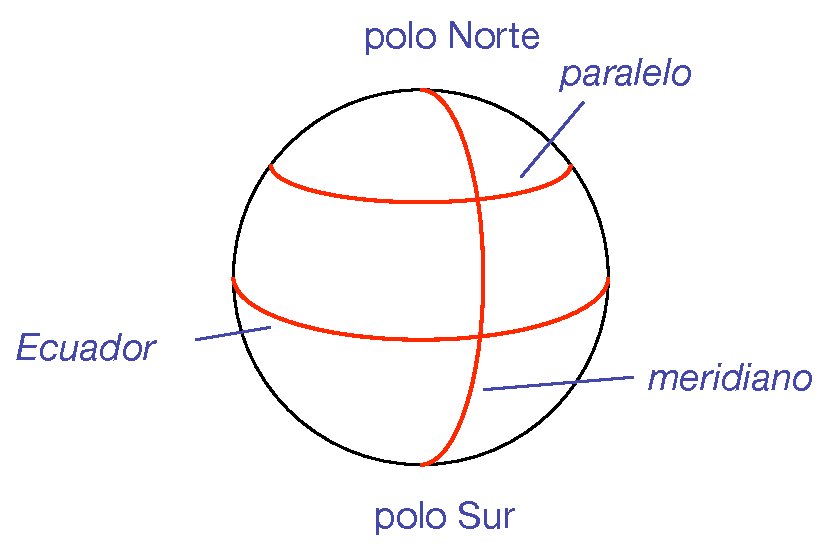
\includegraphics[scale=0.45]{esfera}\\
\caption{Esfera terrestre}
\label{fg:esfera}
\end{center}
\end{figure}


%-------------------------------------------------------------
\subsection{Coordenadas geográficas}

\index{coordenadas|textbf}
\index{coordenadas!geográficas}
\index{coordenadas!latitud|textbf}
\index{coordenadas!longitud|textbf}

%···················································································
\subsubsection{Latitud y longitud}

\index{latitud|textbf}
\index{longitud|textbf}
\index{meridiano!de referencia|textbf}
 \index{meridiano!primer \textemdash|see{meridiano de referencia}}
 \index{meridiano!origen|see{meridiano de referencia}}
 \index{meridiano!de Greenwich} 
 
 \index{Norte}
 \index{Sur}
 \index{Este}
 \index{Oeste}
 
Para situar un punto cualquiera en la superficie de la Tierra se utilizan sus dos \emph{coordenadas geográficas} (figura \ref{fg:coordenadas}): 
\begin{itemize}
\item La \emph{latitud} es el arco de meridiano comprendido entre el ecuador y el punto. Se mide en grados y minutos%
\footnote{Un grado se divide en sesenta minutos, y un minuto en sesenta segundos. Actualmente se prefiere usar fracciones decimales de minuto en vez de segundos. Por ejemplo, 38º 37’ 42” =  38º 37,7’. }
hacia el Norte o hacia el Sur, y su valor está comprendido entre 0º y 90º. 
\item La \emph{longitud} de un punto es el arco de ecuador comprendido entre un \emph{meridiano de 
referencia} o \emph{primer meridiano} y el meridiano que pasa por el punto. Se mide igualmente en grados y minutos, hacia el Este o hacia el Oeste, y su valor está comprendido entre 0º y 180º. Al no haber ningún meridiano que se presente de forma natural como origen para la medida de la longitud, se adopta como meridiano de referencia uno cualquiera, atendiendo a razones de conveniencia. Por convenio internacional el primer meridiano es el \emph{meridiano de Greenwich}, que pasa por el observatorio situado en la ciudad inglesa de ese mismo nombre.%
\footnote{Antiguamente cada país usaba un meridiano de referencia propio. En España se han utilizado como tales los de  la isla del Hierro (punta Orchilla), San Fernando o Cádiz y Madrid, entre otros.} %
\end{itemize}

\begin{figure}[hbtp]
\begin{center}
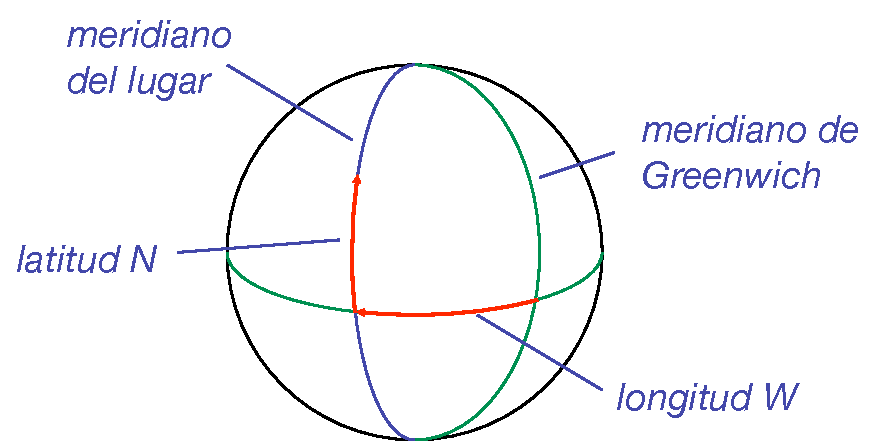
\includegraphics[scale=0.45]{coordenadas}\\
\caption{Coordenadas geográficas}
\label{fg:coordenadas}
\end{center}
\end{figure}

Generalmente se usan las abreviaturas $l$ y $L$, respectivamente, para la latitud y la longitud,%
\footnote{También se usan los símbolos $\phi$ y $\lambda$, respectivamente, para la latitud y la longitud.} 
 y N, S, E y W para las direcciones de los puntos cardinales Norte, Sur, Este y Oeste. La situación de un punto se indica mediante su latitud y longitud, en este orden. Los minutos se escriben generalmente con dos cifras. Normalmente se dan las coordenadas con décimas de minuto, siempre que la situación haya sido obtenida con suficiente precisión. 
 
 \begin{ejemplo}
La latitud del faro del Estacio es \mbox{37º 44,5’ N}, y su longitud \mbox{0º 43,4’ W}. 
Por tanto, su situación es \mbox{37º 44,5’ N 0º 43,4’ W.} 
\end{ejemplo}

%···················································································
\subsubsection{Diferencias de latitud y longitud}

\index{latitud!diferencia}
\index{longitud!diferencia}
 
La \emph{diferencia de latitud} $\Delta l$ entre dos puntos es la resta algebraica de sus latitudes, considerando las latitudes Norte como positivas y las latitudes Sur como negativas. La \emph{diferencia de longitud} $\Delta L$ entre dos puntos es la resta algebraica de sus longitudes, considerando las longitudes Este como positivas y las longitudes Oeste como negativas.%
\footnote{Seguimos aquí el convenio de la Unión Astronómica Internacional (UAI). En algunos manuales de navegación se sigue el convenio contrario, es decir se consideran positivas las longitudes Oeste. El convenio de signos de la UAI tiene ventajas en los cálculos de horas y de estima analítica (ver capítulo \ref{ch:estima}).}

\begin{ejemplo}
La diferencia de latitud y longitud entre el faro del Estacio  y el bajo de En Pou, en el freu grande de Ibiza, situado en
\mbox{38º 48,3' N 1º 25,1' E},  es: 

\[
\begin{array}{lll}
\mbox{Bajo de En Pou}       & +38º \, 48,3’ \:  \mathrm{N}   &   +1º \, 25,1’ \: \mathrm{E}  \\
\mbox{Faro del Estacio}      & +37º \, 44,5’  \: \mathrm{N}   &   -0º  \,43,4’   \:  \mathrm{W}  \\
\hline
 \mbox{Diferencia}               & + \;\;1º  \, 03,8’ \: \mathrm{N}   &    +2º \, 08,5’  \: \mathrm{E} 
\end{array}
\]

Por tanto, el bajo d’En Pou está 1º 03,8’ al Norte y 2º 08,5’ al Este del faro del Estacio. 
\end{ejemplo}

%-------------------------------------------------------------
\subsection{Dirección y distancia }

%···················································································
\subsubsection{Medida de direcciones}

\index{dirección}
\index{rumbo|textbf}
\index{línea!loxodrómica|textbf}

Los marinos miden la dirección de una línea por medio del ángulo que forma con una dirección de referencia. Algunos de estos ángulos tienen un nombre específico. En particular, el ángulo que forma la dirección que sigue un barco con la dirección Norte se llama \emph{rumbo}.  Los rumbos se miden de 0º a 360º a partir del Norte,  en el sentido de las agujas del reloj (figura \ref{fg:rumbo}).

\begin{figure}[hbtp]
\begin{center}
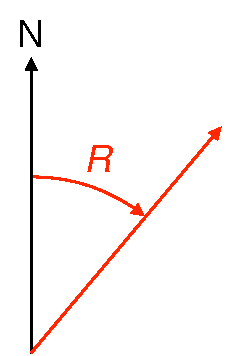
\includegraphics[scale=0.45]{rumbo}\\
\caption{Rumbo}
\label{fg:rumbo}
\end{center}
\end{figure}

Las líneas que forman un ángulo constante con los meridianos (es decir con el Norte) se llaman \emph{líneas loxodrómicas}. Los barcos suelen seguir líneas loxodrómicas en su navegación, ya que para ello basta con mantener un rumbo constante.

%···················································································
\subsubsection{Medida de distancias}

\index{distancia}
\index{distancia!ortodrómica|textbf}
\index{distancia!loxodrómica!textbf}
\index{milla náutica|textbf}
\index{cable|textbf}
 
La unidad de distancia que se usa en navegación es la \emph{milla náutica }($M$),%
\footnote{No existe un acuerdo general sobre el símbolo que se debe usar para la milla náutica. El símbolo $M$ es el recomendado por la Oficina Internacional de Pesos y Medidas.}
 que mide 1852~m, valor aproximadamente igual a la longitud media de 1 minuto de arco de meridiano.%
\footnote{El aplanamiento de la Tierra hace que la longitud de 1' de meridiano varíe ligeramente con la latitud, de manera que su valor es de unos 1843~m en el ecuador, y unos 1861~m en los polos.}

La distancia más corta entre dos puntos situados en una superficie esférica es igual a la longitud del arco de círculo máximo que los une. Su valor se llama \emph{distancia ortodrómica}. Sin embargo, en muchos casos la distancia se mide sobre la línea loxodrómica que une los dos puntos. En este caso se habla de\emph{ distancia loxodrómica}, o \emph{distancia} a secas. En distancias cortas (de menos de 500 millas) no hay error apreciable al medir la distancia loxodrómica en vez de la ortodrómica. 

\begin{ejemplo}
La distancia (ortodrómica) entre el puerto Tomás Maestre, en La Manga, y el Freu Grande de Ibiza es de 119,8~M.. La distancia loxodrómica  entre estos dos puntos es de 120,2~M. Como puede verse, la diferencia no es significativa para distancias de este orden. 

Por otra parte, la distancia ortodrómica entre Vigo y  Nueva York es de 2861~M, mientras que la distancia loxodrómica correspondiente es de 2945~M. Para grandes distancias, por tanto, la diferencia es importante.
\end{ejemplo}

Las distancias menores que una milla se miden en metros, aunque en ocasiones todavía se usa como unidad de medida el \emph{cable}, que equivale a la décima parte de una milla, es decir 185,2~m.

%-------------------------------------------------------------
\subsection{Elipsoide de referencia y datum}

\index{geoide|textbf}
\index{elipsoide|textbf}
\index{elipsoide!de referencia}
\index{datum}
\index{datum!europeo (Potsdam)}
\index{datum!horizontal|textbf}

\index{sistema geodésico mundial|see{WGS84}}
\index{World Geodetic System|see{WGS84}}
\index{WGS,WGS84|textbf}
 
El hecho de que la Tierra no sea perfectamente esférica afecta a la forma de medir la latitud y la longitud. La forma real de la Tierra, suponiendo que toda su superficie estuviera ocupada por los océanos, es una figura geométrica irregular denominada \emph{geoide}. Para calcular las coordenadas geográficas de un punto se aproxima el geoide por un \emph{elipsoide de revolución}, figura que se obtiene al hacer girar una elipse sobre uno de sus ejes (en este 
caso el eje menor). Al ser el geoide irregular, el elipsoide que mejor se ajusta a la forma de la Tierra es diferente para cada zona de la Tierra, y ello ha dado lugar a la utilización de distintos \emph{elipsoides de referencia} por los servicios cartográficos e hidrográficos de los distintos países. Se denomina \emph{datum horizontal} al conjunto de parámetros que se utilizan para determinar las coordenadas geográficas en una zona determinada, a partir de un elipsoide de referencia. 

En Europa se solía usar hasta hace pocos años el llamado \emph{datum europeo}, basado en un elipsoide internacional que se ajusta con el geoide en Potsdam (Alemania). En otros continentes se usan otros datos, como el datum de Norteamérica, el de la India o el de Tokio. Todos ellos han sido sustituidos por el \emph{ sistema geodésico internacional} (\emph{world geodetic system}), más conocido por las siglas WGS84. Este sistema de referencia está ajustado de forma que permite calcular las coordenadas geográficas de puntos situados en cualquier lugar del globo con un error mínimo. 
Las diferencias entre las coordenadas calculadas con respecto a uno u otro datum son pequeñas, generalmente inferiores a 0,1’. Estas diferencias no son significativas cuando se usan métodos poco precisos para calcular la situación de un punto, pero cuando se usan métodos de navegación basados en satélites, que permiten determinar la situación con una precisión de algunos metros, es necesario tenerlas en cuenta. Las cartas españolas, cuando están basadas en el datum europeo,  suelen indicar la diferencia entre las situaciones marcadas en la carta y las referidas al sistema WGS84 (véanse los capítulos \ref{ch:cartas} y \ref{ch:gps}). 

%-------------------------------------------------------------
\subsection{El campo magnético terrestre}
 
\index{Tierra!campo magnético|textbf}
\index{polos!magnéticos}
\index{polos!polo Norte!magnético}
\index{polos!polo Sur!magnético}

\index{declinación|textbf}
\index{declinación!magnética}
\index{declinación!incremento anuo}
\index{declinación!decremento anuo}
\index{variación magnética|see{declinación}}

\index{Norte}
\index{Norte!geográfico}
\index{Norte!verdadero|textbf}
\index{Norte!magnético|textbf}

\index{meridiano|textbf}
\index{meridiano!inferior}
 
La Tierra tiene un campo magnético de intensidad apreciable, orientado aproximadamente en dirección Norte-Sur. Se llama \emph{Norte magnético} a la dirección hacia la que se orienta espontáneamente un imán o una aguja imantada (es decir, una brújula) por efecto del campo magnético terrestre.

El ángulo que forma el Norte magnético con el Norte geográfico o \emph{Norte verdadero} se llama \emph{declinación} o \emph{variación magnética} (figura \ref{fg:declinacion}). Su valor se mide en grados, y es positivo (NE) cuando el Norte magnético está hacia el Este del Norte verdadero, y negativo (NW) cuando el Norte magnético está al Oeste del verdadero. El valor de la declinación se suele representar mediante el símbolo $d_{m}$ o $\delta$. 

La declinación magnética, y por tanto la dirección del Norte magnético, varía para cada lugar de la Tierra. Además, su valor cambia con el tiempo, llamándose \emph{incremento} o \emph{decremento anuo} la diferencia de valor de la declinación entre un año y el siguiente. Las cartas y otros documentos náuticos (ver capítulo \ref{ch:cartas}) proporcionan el valor de la declinación y su diferencia anua en las zonas que cubren. 

\begin{ejemplo}
La declinación magnética en las cercanías del cabo de la Nao en 2004 era de 1º W, con una diferencia anual de 7’ E. En este caso la declinación es negativa y la diferencia es positiva. Si queremos calcular el valor de la declinación en 2009 efectuaremos las siguientes operaciones: 
\[ 
\begin{array}{lcll}
\mbox{Valor en 2004 } &   = &  -1º \, 00’ \: \mathrm{(W) } \\
\mbox{Diferencia}         &   = &   +0º \, 35’ \: \mathrm{(E)}  &(\mbox{5 años} \times 7' )\\
\mbox{Valor en 2009}  &  = &   -0º \, 25’ \: \mathrm{(W)} & \approx -0,5º 
\end{array}
\]
\end{ejemplo}

El valor de la declinación se suele dar en grados y minutos enteros o en grados y décimas de grado. 

%===================================
\section{El tiempo}

\index{tiempo|textbf}
\index{segundo|textbf}
\index{sistema internacional de unidades}
\index{SI|see{sistema internacional de unidades}}

 
La medida precisa del tiempo es de gran importancia para la navegación. El tiempo transcurrido desde la última situación nos permite calcular la distancia recorrida, si conocemos la velocidad del barco. La determinación exacta del instante de las observaciones es fundamental en navegación astronómica, y la navegación por satélite hace uso de relojes atómicos de gran precisión para medir el tiempo que tardan las señales radiadas en llegar al observador. Por tanto, el navegante debe ser capaz de conocer la hora en todo momento con la precisión necesaria para el tipo de navegación que esté efectuando. 

Desde la antigüedad más remota se ha medido el tiempo a partir de la observación de los fenómenos astronómicos más evidentes: la rotación de la Tierra, a partir de la cual se define la duración del día y su división en horas, minutos y segundos, y su traslación alrededor del Sol, cuya duración es de un año. La observación de las fases de la Luna dio origen, por su parte, a la semana y el mes. 

A medida que se dispuso de relojes e instrumentos astronómicos más precisos se observó, sin embargo, que estos fenómenos astronómicos presentan irregularidades. Ello dio lugar a definiciones más precisas de las unidades de tiempo, hasta llegar a la época actual, en que la medida del tiempo se basa en la observación de fenómenos atómicos de 
una gran regularidad. Actualmente todas las medidas de tiempo se refieren al Sistema Internacional de unidades (SI),  cuya unidad fundamental es el \emph{segundo} ($s$). Esta unidad se define a partir de la frecuencia de la radiación emitida por un átomo de Cesio.%
\footnote{La duración del segundo se define como $9\,192\,631\,770$ períodos de la radiación correspondiente a la transición entre los dos niveles hiperfinos del átomo de Cs\textsuperscript{133}. }
Para los usos prácticos, sin embargo, se mantienen las unidades de tiempo tradicionales, estableciéndose formalmente su relación con la unidad fundamental: 

\begin{tabular}{lcl}
1 minuto &= &60 segundos\\
1 hora     &= &60 minutos\\
\end{tabular}

Normalmente se da la hora del día en horas y minutos, o en horas, minutos y segundos. Se suelen dar los valores respectivos separados por sus abreviaturas (h, m, s) o por el signo “:” (dos puntos). Cuando se dan sólo las horas y minutos se pueden escribir con las cuatro cifras respectivas sin separación. 

\begin{ejemplo}
Las siguientes expresiones se refieren a la misma hora: 

\begin{center}
\begin{tabular}{lll}
3h 45m & 03:45 & 0345 \\
\end{tabular}
\end{center}
\end{ejemplo}

\index{sistema de referencia de tiempo}
\index{sistema de referencia de tiempo!\textemdash|seealso{tiempo solar, tiempo solar medio, tiempo universal}}

La expresión de la hora del día está sujeta a un \emph{sistema de referencia de tiempo}. A continuación se describen de forma resumida los sistemas de referencia más usados en navegación. 

%-------------------------------------------------------------
\subsection{Tiempo solar}

\index{tiempo!solar}
\index{día!solar}

El tiempo solar se mide a partir del movimiento aparente del Sol. Un \emph{día solar} es el tiempo que transcurre entre dos pasos sucesivos del Sol por el meridiano de un lugar. El día solar se divide en 24 \emph{horas solares}, y la \emph{hora solar} es el número de horas solares transcurridas desde el paso del Sol por el meridiano inferior del lugar. 

El tiempo solar no se utiliza apenas, ya que la forma elíptica de la órbita de la Tierra en torno al Sol, la inclinación del eje de la Tierra sobre el plano de esa misma órbita (denominado \emph{plano de la eclíptica}), y algunas otras irregularidades hacen que la duración del día solar presente notables variaciones a lo largo del año.%
\footnote{La diferencia entre el día solar más corto y el más largo es de algo más de 30~minutos.}

%-------------------------------------------------------------
\subsection{Tiempo solar medio}

\index{tiempo!solar medio}
\index{día!solar medio}
\index{hora!solar media}
\index{hora!civil}

Para evitar las irregularidades del tiempo solar se utiliza el \emph{tiempo solar medio}, basado en la duración media del día solar y en la aproximación del movimiento real de la Tierra por otro imaginario en el que se considera que la órbita de la Tierra es circular y su eje es perpendicular al plano de la eclíptica. El movimiento aparente del Sol en esta aproximación se denomina \emph{Sol medio}, y es regular a lo largo del año. De esta manera se define el \emph{día 
solar medio} como la duración media del día solar. El día solar medio tiene una duración aproximadamente igual a 24 horas. La \emph{hora solar media} u \emph{hora civil} de un lugar es el tiempo transcurrido desde el paso del Sol medio por el meridiano inferior del lugar, o lo que es lo mismo desde la medianoche del día solar medio. 

%-------------------------------------------------------------
\subsection{Tiempo universal}

\index{tiempo!universal}
\index{hora!universal|seealso{tiempo universal}}
\index{hora!civil!de Greenwich|seealso{tiempo universal}}
\index{TU|see{tiempo universal}}
\index{UT|see{tiempo universal}}

Como el Sol pasa en distintos momentos por el meridiano de cada lugar, la hora civil será diferente para cada lugar de la Tierra, aunque todos los lugares situados en el mismo meridiano tienen la misma hora civil. Para evitar los inconvenientes que ello acarrea conviene definir un \emph{tiempo universal} que sirva de referencia para toda la Tierra. Por convenio internacional se toma como tiempo universal el tiempo solar medio del meridiano de Greenwich, u \emph{hora civil de Greenwich}. Para designar el tiempo universal se usan las abreviaturas TU o UT (\emph{universal time}).%
\footnote{Está en desuso la abreviatura GMT (\emph{Greenwich Mean Time}) que se usaba para designar el tiempo universal.}

%...................................................................................
\subsubsection{Hora civil y hora universal}

\index{hora!civil}
\index{hora!universal}

La hora civil de los lugares que están situados en meridianos diferentes del de Greenwich está relacionada con la hora universal por la longitud. Como el día solar medio dura 24~horas, y esto equivale a una rotación de 360º, la Tierra gira 15º ($= 360/24$) cada hora. En consecuencia, los lugares que están 15º al Oeste del meridiano de Greenwich tienen 
una hora civil que es una hora anterior a la hora universal, y así sucesivamente. En general, la fórmula que relaciona la hora civil de un lugar (HcL) con la hora universal (TU) es: 
\begin{equation}
\mathrm{HcL} = \mathrm{TU} + \Lambda
\end{equation}
donde $\Lambda$ es el equivalente en tiempo de la longitud, 
\begin{equation}
\Lambda = \frac{L}{15}
\end{equation}
$L$ se expresa en grados y fracciones de grado. Hay que tener en cuenta el convenio de signos para la longitud (positiva al Este) para aplicar esta fórmula. 

\begin{ejemplo}
La hora civil en Cedeira (43º 39,7’ N 8º 3,2’ W) cuando son las 15h 37m TU es 
\[
\begin{array}{lcrr}
  \mathrm{TU} &  =  &   23 & 58 \\
  \Lambda        &  =  &   -00 & 32\\ \cline{3-4}
  \mathrm{HcL} &   = &   15 &05\\
\end{array}
\]
El valor de $\Lambda$ se calcula dividiendo 8,05 ($\mathsf{= 8+3.2/60}$) por 15. El resultado es $0.54$ horas, es decir 32 minutos ($\mathsf{=0.54 \cdot 60}$). El valor es negativo por ser la longitud Oeste. 
\end{ejemplo}

Hay que tener en cuenta que la hora civil en un lugar determinado puede corresponder a una fecha distinta de la correspondiente a la hora universal. 

\begin{ejemplo}
La hora civil en Mahón (39º 52,1’ N 4º 18,6’ E) cuando son las 23h 58m TU del día 8 de abril es: 
\[
\begin{array}{lcrrl}
  \mathrm{TU} &  =  &   23 & 58 \\
  \Lambda        &  =  &   +00 & 17\\ \cline{3-4}
  \mathrm{HcL} &   = &   00 & 15 & \mbox{(día 9 de abril)}\\
\end{array}
\]
es decir, las 00h 15m del día siguiente. 
\end{ejemplo}

%-------------------------------------------------------------
\subsection{Tiempo universal coordinado}

\index{tiempo!universal coordinado|textbf}
\index{UTC|see{tiempo universal coordinado}}
\index{TUC|see{tiempo universal coordinado}}
\index{hora!universal}
\index{hora!UTC}

El tiempo universal coordinado (TUC o UTC, \emph{Universal Time Co-ordinated}) se basa en el empleo de relojes atómicos, ajustados de tal manera que su valor no difiera en más de 0,9~s del tiempo universal basado en observaciones astronómicas. El TUC es la base de la hora oficial en todos los países del mundo. 

En lo sucesivo consideraremos que el TU y el TUC son equivalentes. 

%-------------------------------------------------------------
\subsection{Hora legal}

\index{hora!legal}
\index{huso horario|textbf}
\index{zona horaria}
\index{zona horaria!\textemdash|seealso{huso horario}}

El hecho de que la hora civil de lugares próximos sea diferente hace su uso poco práctico para la vida diaria. Para evitar este inconveniente se suele adoptar una misma \emph{hora legal} para una zona de la Tierra. Con este fin se divide la superficie terrestre en 24 \emph{husos horarios} de 15º de longitud cada uno, centrados en los meridianos 0º, 15º, etc. (figura \ref{fg:husos}). 

\begin{figure}[hbtp]
\begin{center}
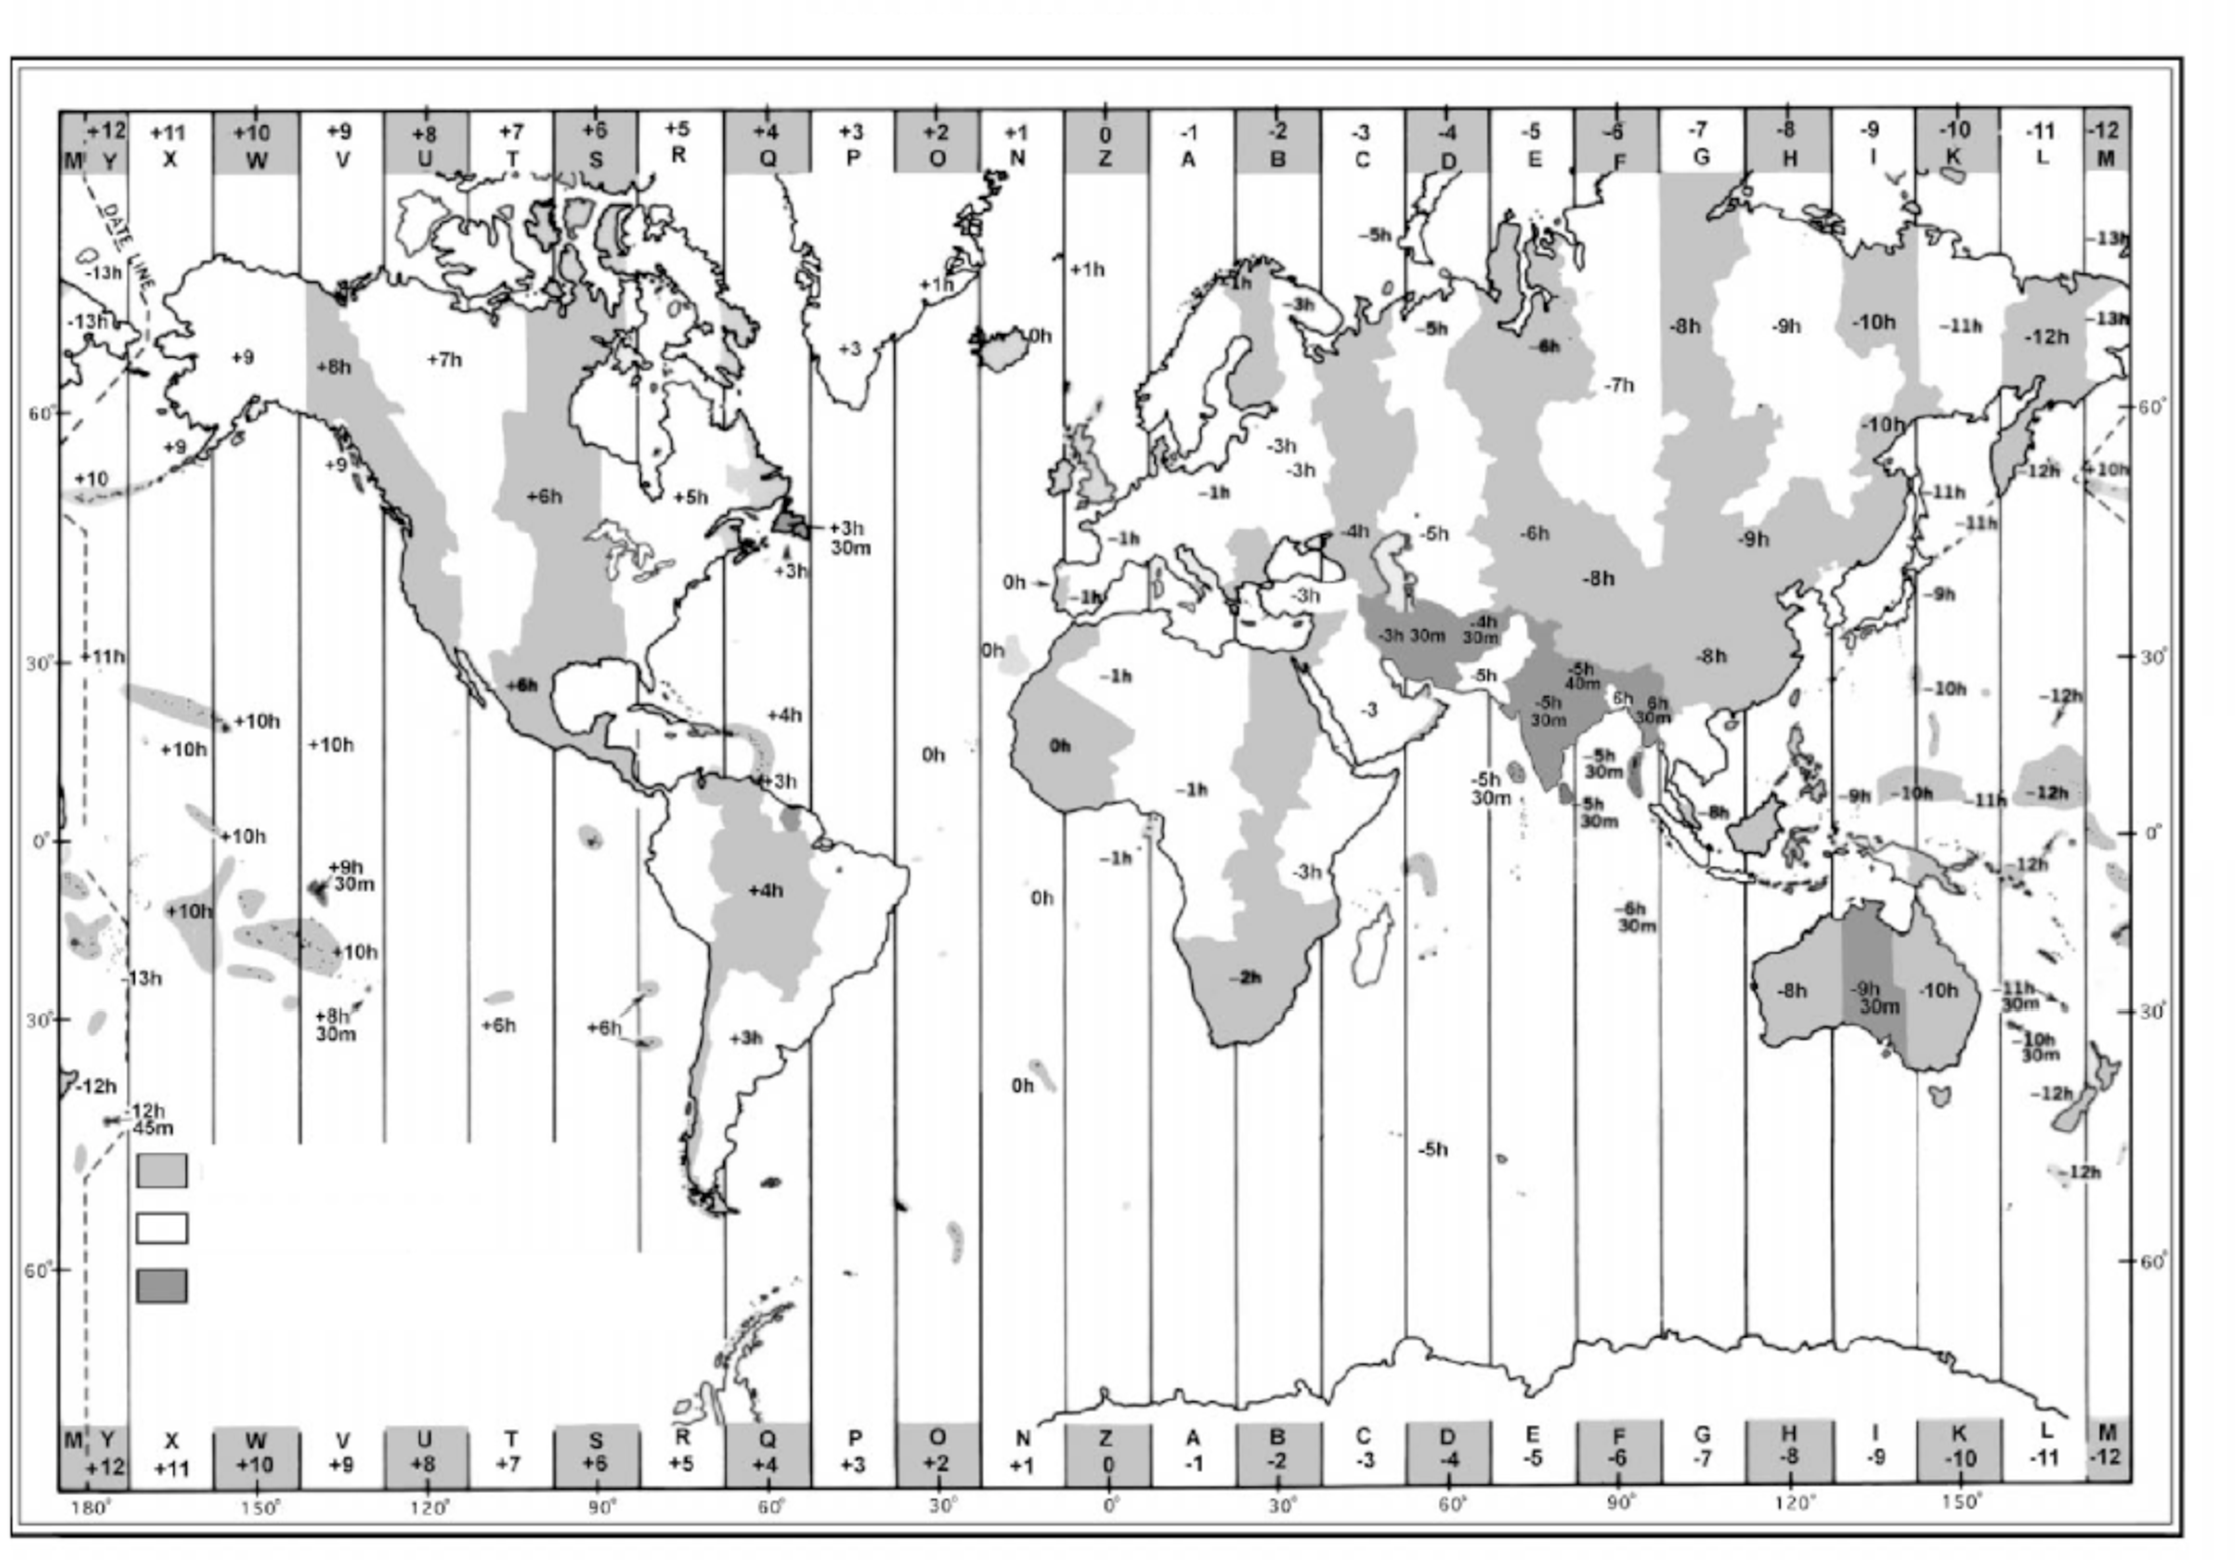
\includegraphics[width=\textwidth]{husos}\\
\caption{Husos horarios y zonas de hora legal}
\label{fg:husos}
\end{center}
\end{figure}

Todos los lugares que están en un mismo huso horario tienen la misma hora legal. En algunas partes del mundo se usan zonas horarias que no coinciden exactamente con los husos horarios. Por ejemplo, toda la parte peninsular de España está incluida en la zona 0, aunque estrictamente hablando la parte occidental de Galicia pertenece al huso -1. Las Islas Canarias se encuentran en su totalidad en la zona -1. 

La hora legal (Hl) de un lugar está relacionada con la hora universal por la ecuación: 
\begin{equation}
\textrm{Hl} = \mathrm{TU} + Z
\end{equation}
donde $Z$ es la zona o huso horario en que se encuentra el lugar. 

En alta mar el valor de Z es 
\begin{equation}
Z = \mathrm{entero}\left(\frac{L}{15}\right)
\end{equation}
pero en puerto y en aguas territoriales la hora legal será la que corresponda a la zona horaria del lugar en que nos encontremos.

La función \textit{entero} da el valor entero redondeado más próximo a su argumento.  Por ejemplo, 
$\mathrm{entero}(1,2) = 1$, pero $\mathrm{entero}(1,7) = 2$.

\begin{ejemplo}
Se desea obtener la hora legal en un lugar situado en \mbox{40º 35,0’\:N} 37º 12,7’ W cuando son las 0235 TU.

En primer lugar se calcula la zona horaria:
\[ Z  = \mathrm{entero}(-37.21/15)  =  \mathrm{entero}(-2.48) =  -2 \]
teniendo en cuenta que $ 37º 12.7’ = 37+12.7/60 = 37.21º $.

 La hora legal se calcula de la siguiente forma:
\[
\begin{array}{lcrr}
  \mathrm{TU} & =  &  02 & 35 \\
  Z                     & = &   -02 &00 \\ \cline{3-4}
  Hl                    & = & 00 & 35
\end{array} 
\]

\end{ejemplo}

%...................................................................................
\subsubsection{Línea de cambio de fecha}

\index{línea!de cambio de fecha}

El meridiano 180º puede considerarse indistintamente Este u Oeste. Por tanto, se puede considerar que la hora en el mismo es 12 horas anterior o 12 horas posterior al TU. Para resolver esta ambigüedad se conviene en cambiar la fecha al llegar a dicho meridiano, de forma que cuando se va hacia el Este se cuenta un día menos y cuando se va hacia el Oeste 
se cuenta un día más. 

Para evitar los problemas que surgen en las escasas tierras que se encuentran sobre este meridiano, se definió una línea internacional de cambio de fecha que se aparta ligeramente del meridiano 180º en las zonas de tierra (figura \ref{fg:husos}). 

\begin{ejemplo}
Cuando son las 15\,30 TU del día 8 de abril, en el meridiano 175º E son las 03\,30 del
día 9, mientras que en el meridiano 175º W son las 03\,30 del día 8. 
\end{ejemplo}

%-------------------------------------------------------------
\subsection{Hora oficial}

\index{hora!oficial\textbf}
\index{hora!de Europa central (CET)}
\index{horario!de verano}
\index{horario!de invierno}
\index{CET}

En algunos países se modifica la hora legal por motivos políticos o económicos, durante todo el año o durante algunos meses. La \emph{hora oficial} en estos países es igual a la hora legal corregida con un adelanto o retraso: 
\begin{equation}
\mathrm{Ho} = \mathrm{Hl} + C
\end{equation}
donde $C$ es la corrección oficial (adelanto o retraso). En España $C$ es igual a 1~hora en invierno
 y 2horas en verano.%
\footnote{La hora oficial en la España peninsular es la denominada CET (\emph{Central Europe Time}), que es oficial también en la mayoría de los países de Europa Occidental. El horario de verano comienza el último domingo de marzo a las 0100 TU, y termina el último domingo de octubre a la misma hora (0100 TU). En Canarias la correción es la misma, y el cambio de hora se efectúa al mismo tiempo que en la península. Como las islas Canarias están en el huso -1, la hora oficial en Canarias es siempre una hora menos que en la Península.}

%-------------------------------------------------------------
\subsection{El reloj de bitácora}

\index{reloj de bitácora}
\index{hora!del reloj de bitácora (HRB)}
\index{HRB}

El \emph{reloj de bitácora} es el que se usa a bordo de un barco para marcar la hora. Se suele poner en hora con la hora oficial cuando se navega cerca de la costa, o con la hora legal cuando se navega en alta mar. La expresión \emph{hora del reloj de bitácora} (HRB) se refiera a la hora que marca el reloj de bitácora, y es por tanto equivalente a hora oficial u hora legal, según los casos. 

%-------------------------------------------------------------
\subsection{La fecha y el calendario}

\index{fecha}
\index{calendario}

La determinación de la fecha se basa, como es sabido, en el movimiento de traslación de la Tierra alrededor del Sol, cuyo período, denominado \emph{año trópico}, tiene una duración de 365,2425 días aproximadamente. Para ajustar la duración del año a un número entero de días completos se usan las reglas del \emph{calendario gregoriano}, por las cuales se añade un día (el 29 de febrero) a determinados años, denominados \emph{años bisiestos}. Son bisiestos los años cuyo número es múltiplo de 4, excepto los múltiplos de 100 que no lo son de 400 (por ejemplo, el año 2000 fue bisiesto, pero no lo fueron los años 1700, 1800 ni~1900).
